\documentclass[10pt]{article}

\usepackage{polski}
\usepackage{graphicx}
\usepackage{hyperref}
\graphicspath{{images/}}

\usepackage{geometry}
\newgeometry{tmargin=4cm, bmargin=4cm, lmargin=3.2cm, rmargin=3.2cm} 

\usepackage{fancyhdr}
\pagestyle{fancy}

 

\begin{document}


\begin{titlepage}
\begin{center}

    \LARGE \textsc{Politechnika Wrocławska}\\
    \vspace*{0.2cm}
    \Large \textsc{Wydział Informatyki i Telekomunikacji}\\
    \vspace*{0.4cm}
    \centering
\includegraphics[width=0.2\textwidth]{WITlogo.png}\
    \vspace*{0.2cm}
    \vspace*{2cm}

    \centerline{\rule{\textwidth}{1.2pt}}
    \vspace*{0.4cm}
    \Huge \textbf{Regresja danych dotyczących ilości miejsc pracy}
    \centerline{\rule{\textwidth}{1.2pt}}
    \vspace*{1cm}
    \Large Sprawozdanie z laboratorium\\
    \vspace*{0.2cm}
    \textbf{Wojciech Gruba}\\
    \vspace*{0.1cm}
    \Large nr albumu: \textbf{259170}
    \vspace*{0.1cm}
    kierunek: \textbf{Informatyka Stosowana}



    \vspace*{\fill}
    \Large \textit{07 czerwca 2022}

\end{center}

\end{titlepage}


\begin{abstract}

Praca przedstawia program do obliczania regresji liczby zajętych miejsc pracy w wybranych rodzajach przemysłu oraz regionu w jakim dana firma sie znajduje. Program działa dzięki danym pobranym ze strony data.ny.gov.
Dane te zostały oczyszczone ze zbędnych wierszy nieposiadających kompletnych informacji, do danych została dodana kolumna "PrevJobs" zawierająca informację o stanie miejsc pracy sprzed roku. Następnie ze zbioru danych zostały wylosowane wiersze mające służyć predykcji miejsc pracy na podstawie daty, rodzaju przemysłu oraz regionu. W programie zostały wykorzystane modele regresji liniowej, model customowy wtkorzystujący funkcję curve fit z modułu scipy oraz SVR z modułu sklearn. Następnie dzięki funkcjom mean squared error oraz mean absolute percentage error z modułu sklearn zostały obliczone błędy kwadratowe oraz procentowe modeli regresji. Na zakończenie pracy program wyświetla wykres z oryginalnymi wartościami oraz wartościami wyliczonymi dzięki modelom regresji. 

\end{abstract}

\section{Wstęp -- sformułowanie problemu}
\label{sec:wstep}

Autor chce przewidzieć ilość miejsc pracy w poszczególnych rejonach oraz typach przemysłu. Pozwoli mu to na ocenę rozwoju poszczególnych typów przemysłu w przyszłych latach.

\section{Opis danych}

Wielkość datasetu 2079 wierszy.
    Kolumna "Year" - zmienna całoliczbowa, określa rok z którego dane zostały pobrane.\\
    Zbiór wartości: 2012 - 2020
    
    Kolumna "Region" - zmienna kategoryczna, określająca nazwę lokalizacji dla jakiej dane zostały przygotowane.\\
    Zbiór wartości to Capital Region, Finger Lakes, Mid-Hudson, New York City, North Country, Southern Tier, Mohawk Valley, New York, Central New York
    
    Kolumna "NAICS code" - zmienna całoliczbowa, Północno-amerykański system klasyfikacji przemysłu.\\
    Zbiór wartości: 11-99
    
    Kolumna "Industry" - zmienna kategoryczna, określająca nazwę przemysłu. \\
    Zbiór wartości: Retail Trade, Wholesale Trade, Finance and Insurance, Arts, Accomodation and Food Services, Information, Agriculture, Mining, Other, Technical Services, Educational Services, Goverment, Transportation, Real Estate, Administrative and Support and Waste Managment, Utilites, Health Care, Construction, Manufacturing, Managment of Companies and Enterprises, Unclassifed.
    
    Kolumna "Jobs" - zmienna całoliczbowa, określająca ilość wszystkich zatrudnionych ludzi w określonym rodzaju przemysłu. \\
    Zbiór wartości: 27 -703,838
    
    
\section{Opis rozwiązania}

Dane dotyczące ilości pracowników zostały pobrane ze strony\\ \url{https://data.ny.gov/Economic-Development/Jobs-By-Industry-Beginning-2012/pxa9-czw8}. Baza została zapisana w postaci ramki danych biblioteki \texttt{Pandas}. Zawiera ona informacje o 3 cechcach określających możliwości zatrudnienia w danych gałęziach przemysłu.
    Po dodaniu wiersza PrevJobs program wybiera wiersze do dalszej pracy.
Kożystając z modeli linear model, SVR oraz własnego modelu regresji, na wybranych danych program wylicza przewidywaną liczbę zatrudnionych pracowników. Następnie dzięki bibliotece matplotlib, prawdziwe i wyliczone dane nanoszone są na wykres i wyświetlane uzytkowikowi. 

\section{Rezultaty obliczeń}

\subsection{Plan badań}
Zbiór danych zostanie podzielony na dwie części: treningową i testową w stosunku 80:20. 


\subsection{Wyniki obliczeń} 
Model wyliczania liczby miejsc pracy można przedstawić następującym wzorem: 
\begin{equation}
\det Jobs = \alpha * Year + \beta * get\_dummies(Region) + \gamma * get\_dummies(Industry) + \delta * PrevJobs 
\label{eq:wzor_wazny}
\end{equation}
gdzie $get\_dummies()$ to funkcja mapująca dane kategoryczne na reprezentację one-hot.

Na rys. \ref{fig:wykres} pokazany jest przykładowy wykres. 
\begin{figure}[!hbt]
\begin{center}
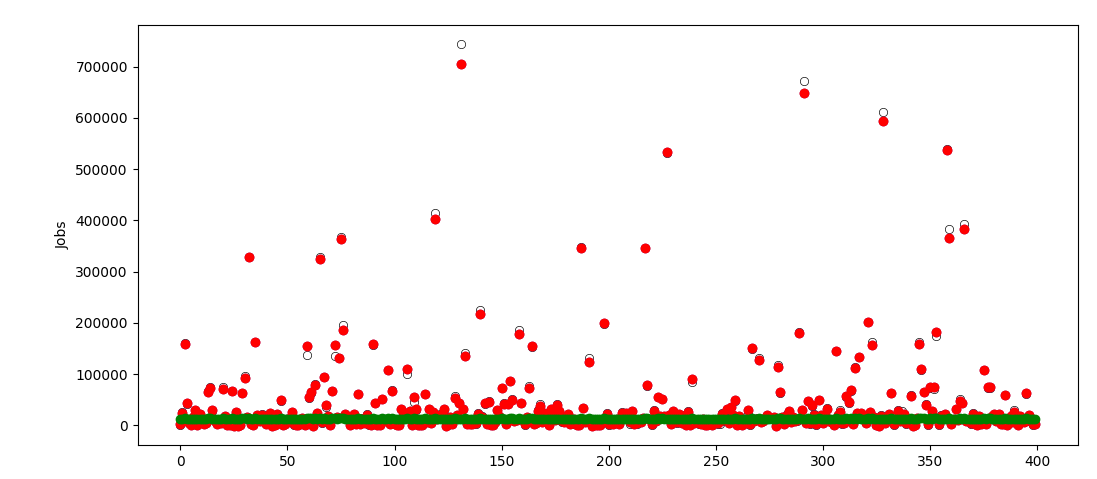
\includegraphics[width=0.8\linewidth]{rys1.png}
\caption{Przewidywane wartości dla modeli}
\label{fig:wykres}
\end{center}
\end{figure}

Funkcje mean squared error oraz mean absolute percentage error z modułu sklearn wyliczają błędy kwadratowe oraz procentowe dla poszczególnych sesji, aby sprawidzć ich skuteczność

\section{Wnioski}
Przedstawiony program pozwala na dobranie optymalnego modelu regresji do przewidzenia ilości zatrudninych ludzi w danej gałęzi przemysłu. Po próbach z różnymi wielkościami danych skuteczność modelu SVR niezależnie od ilości danych wypada najgorzej, natomiast własny model oraz model liniowy przewidują nieznacznie różniące się wartości.
Zależnie od liczby wierszy wziętych do stworzenia modelu, model linowy oraz custom model zazwyczaj osiągają błąd procentowy rzędu 0,5 natomiast SVR rzędu kilku procent.
Wszystkie modele dla danych bez dodatkowej kolumny PrevJobs osiągały błąd procentowy rzędu 20 procent niezależnie od typu modeu.
Model własny potrzebuje danych posiadających kilkaset wierszy aby optymalnie działał, ponieważ liczba kolumn musi być mniejsza niż liczba wierszy, z tego powodu gdy posiadamy dane mające 40 wierszy, model customowy sie nawet nie wykona, a dla wartości rzędu 70 wierszy błąd procentowy będzie wyższy niż dla dużej ilości danych. 

    

\appendix
\section{Dodatek}
Kody źródłowe(utrzymane w konwencji języka Python) umieszczone zostały w repozytorium github:

\noindent \url{https://github.com/wgruba/MSID}.


\end{document}